% Title: Monoids. What, how and why?
% Titulo: Monoides. Que, Como e Por Que?

% Abstract:
% We will learn about Monoids, a concept invented (discovered?) by mathematicians
% that we can leverage to great value in our code and designs.

% The talk is structured in two sessions, in this first one (5/29) we'll learn what
% Monoids are, go through many examples, and write code that creates and uses Monoids. In
% the second session (June maybe?) we will see how we can use Monoids to guide software design.

% Despite the weird name, Monoids are easy to understand, and once you do, you'll
% start finding them everywhere. More importantly, after a little practice
% you'll gain intuition and you'll be able to integrate Monoids in your code and
% designs, obtaining more abstract and reusable results.

% Requirements:
% This is an intermediate level talk. No knowledge of math or functional
% programming is required. I'll assume you can understand simple Scala code.
% In particular, if you don't know what implicit parameters are, spend 10 minutes
% learning about them. You don't need to understand the details of implicit search
% mechanisms or anything like that.


% Resumo:
% Vamos aprender sobre Monoids, um conceito inventado (ou descoberto?) pelos
% matematicos, que nos podemos aproveitar com grandes resultados no nosso codigo e desenhos.

% A palestra esta estruturada em duas sessoes, na primeira (29/05) vamos aprender o
% que sao os Monoids, ver muitos exemplos e escrever codigo que cria e usa
% Monoids. Na segunda sessao (data a confirmar) vamos ver como podemos usar os
% Monoids para guiar o desenho de software.

% Apesar de seu nome estranho, os Monoids sao faceis de entender, e uma vez que os
% entenda, voce vai acha-los em todo lugar. Ainda mais importante, com um
% pouco de pratica, voce vai aprimorar sua intuicao e sera capaz de integrar Monoids no seu
% codigo e desenhos, consiguindo resultados mais abstratos e reusaveis.

% Requerimentos:
% Essa e uma palestra de nivel intermediario. Nao precisa conhecimentos de
% matematica ou programacao funcional. Todos os exemplos serao em Scala, voce devera
% conhecer a linguagem para entende-los. Particularmente, se voce nao sabe o que sao os parametros
% implicitos, gaste 10 minutos aprendedo-os. Nao precisa saber os detalhes dos
% mecanismos de busca de implicitos.

% Bio:

% Depois de quase uma década trabalhando em linguagens imperativas, Sebastian
% abraçou a programação funcional e nunca mais olhou para atrás. Nos últimos oito anos
% ele tem trabalhado nas áreas de data science, infraestrutura de Big Data e
% enterprise software, em linguagens como Scala, Haskell e Clojure. Cuidado!
% O Sebastian vai tentar trazer você para o mundo da programação funcional.


\documentclass{beamer}
\usepackage[english]{babel}
\usepackage[utf8]{inputenc}
\usepackage[T1]{fontenc}
\usepackage{pgfpages}
\usepackage{listings}
\usepackage{color}
\usepackage{ulem} % for \sout
\usepackage{tikz}
\usepackage{amsmath}

\mode<presentation>
{
  \usetheme{Madrid}      % or try Darmstadt, Madrid, Warsaw, ...
  \usecolortheme{default} % or try albatross, beaver, crane, ...
  \usefonttheme{default}  % or try serif, structurebold, ...
  \useoutertheme{default}
  \setbeamertemplate{navigation symbols}{}
  \setbeamertemplate{caption}[numbered]

  % \AtBeginSubsection[]
  % {
  %   \begin{frame}<beamer>\frametitle{OUTLINE}
  %     \tableofcontents[currentsection,currentsubsection]
  %   \end{frame}
  % }

}

\pgfdeclareimage[height=0.5cm]{assoc-logo}{assoc.png}
\logo{\pgfuseimage{assoc-logo}}

\setbeameroption{show notes on second screen}
\setbeamerfont{note page}{size=\tiny}





\title[Monoids]{MONOIDS}
\subtitle{\textit{What}, \textit{How} and \textit{Why}}
\author{Sebastian Galkin}
\institute[@paraseba]{\texttt{@paraseba} \\ \texttt{paraseba@gmail.com}}
\date[Scaladores]{Scaladores - May 2018}
\subject{Talks}

\definecolor{keyword}{rgb}{0,0.38,0}
\definecolor{comments}{rgb}{0.4,0.1,0.1}

\begin{document}
\lstset{
  language=Scala,
  basicstyle={\small\ttfamily},
  keywordstyle=\color{keyword},
  commentstyle={\color{comments}\itshape},
  columns=fullflexible,
  escapechar=~,
  showlines=false,
}


\begin{frame}
  \titlepage
\end{frame}

% Uncomment these lines for an automatically generated outline.
\begin{frame} \frametitle{OUTLINE}

  \note{
    Hoje vamos falar sobre Monoides. Depois de uma breve introducao
    sobre abstracao, vou mostrar que eh um monoide, e um monte de
    exemplos de monoides interesantes. Finalmente vamos ver varios
    casos onde podemos usar monoides para melhorar nosso codigo
    e para resolver problemas concretos dificis.

    Para manter voces acordados, e ter certeca que estao entendendo,
    vou fazer perguntas que completam o material (fixme).

    Podem me interromper se tever duvidas, ou nao entender. Mesmo se o
    que nao entender for o sotaque, me interrompe e com uma mistura de
    portugues, espanhol e ingles vamos nos entender.
  }

  \begin{columns}[c]
    \column{0.6\textwidth}
      \tableofcontents
    \column{0.4\textwidth}
      \rotatebox{45}{\Large \textcolor{blue}{\texttt{There will be quizzes}}}
  \end{columns}
  \begin{block}{}
    \centering
    \Large \textbf{Ask questions as we go!}
  \end{block}
\end{frame}


\begin{frame} \frametitle{ABOUT ME}
  \note {
    Um pouco acerca de mim: faco programacao funcional exclusivamente
    a ums 8 anos. Scala, Haskell, Clojure e outros. Trabalho em data
    science e infrastrutura para big data, mas com alguns periodos de
    software para enterprise. Adoro FP, me faiz sentir inteligente, me
    diverte, me desafia. Nao imagino como seria voltar para a programacao
    imperativa.

    Um problema da FP eh que da medo. Muitas palavras em latim, muitos
    matematicos, um pouco de soberbia... Precisamos mudar isso. FP nao
    eh dificil, so eh diferente. Nao precisa ser matematico, nem genio,
    so ter vontade.

    Se voce quer aprender, ou se voce quer que seu teame aprenda FP? me
    contata. Vamos conversar.
  }

  {\LARGE Sebastian Galkin}

  \begin{itemize}
  \item \alert{Functional Programming} for a while.
  \item Mostly big data and enterprise.
  \item People are still scared of FP.
  \item You or your team want to learn FP?
  \color{blue}\texttt{paraseba@gmail.com}
  \end{itemize}


\end{frame}

\section{Monoids in Code}
\subsection{Abstraction}

\begin{frame} \frametitle{WHAT IS ABSTRACTION?}
  \begin{quote}
\textbf{Abstraction} is the process of extracting the underlying \alert{essence} of a concept,
removing any \alert{dependence} on real world objects, and \alert{generalizing} it so that it
has \alert{wider applications.}\\[2ex] \rightline
  {{\rm --- Wikipedia, \href{https://en.wikipedia.org/wiki/Abstraction_(mathematics)}{\underline{Abstraction (mathematics)}}}}
  \end{quote}

  \note {
    Eu peguei essa cita da pagina da wikipedia dedicada a abstracao em
    matematica. Toma um tempo para ler [esperar 15 segundos].

    Se nao chegou a ler, olha so as partes em vermelho: esencia do conceito,
    dependencias, generalizar, reusar. Sao as mesmas palavras que usamos para
    descreber o que chamamos software de qualidade! Lembre que tirei isso de uma
    pagina que fala de matematica!

    Casualidade? Nao acho.

    Na verdade, o conceito de abstracao que temos na industria de software esta
    muito pouco desenvolvido. A maioria das pessoas quando pensa em abstracao
    pensa em indirecao, ou evitar repeticao de codigo. Mas abstracao nao tem
    nada a ver com isso!
  }
\end{frame}

% \begin{frame} \frametitle{YOU CALL THIS ABSTRACTION?}
%   \begin{quote}
%     I wouldn't really think of abstraction as a mathematical concept. \\[1ex] \rightline
%   {{\rm --- Fishtoaster,
%       \href{https://softwareengineering.stackexchange.com/questions/16070/what-is-abstraction}{\underline{SE Stack Exchange}}}}
%   \end{quote}

%   \begin{quote}
%     A programming abstraction is a simplified model of a problem. \\[1ex] \rightline
%   {{\rm --- C. Ross,
%       \href{https://softwareengineering.stackexchange.com/questions/16070/what-is-abstraction}{\underline{SE Stack Exchange}}}}
%   \end{quote}

%   \note {
%     Vamos ver o que pensa o pessoal da ingeniaria de software sobre abstracao.
%     [esperar 15 segundos]

%     ``Abstracao nao eh um conceito matematico''???

%     ``simplified model of a problem''???

%   }

%   \pause

%   \begin{block}{These are not abstraction}
%   \begin{itemize}
%     \item Indirection.
%     \item Inheritance.
%     \item Factoring out common code to a function.
%     \item Passing to functions only what they need.
%   \end{itemize}
%   \end{block}

%   Really, how abstract is your code?

%   \begin{center}
%     \LARGE
%     \bfseries
%   We suck at abstraction!
%   \end{center}
% \end{frame}

\begin{frame} \frametitle{STANDING ON THE SHOULDERS OF GIANTS}
  Mathematicians are the \alert{masters of abstraction.}
  \begin{itemize}
  \item Maximize generality.
  \item Analogies and analogies between analogies.
  \item Reusing whole theories.
  \item Finding ``the right'' level of abstraction.
  \end{itemize}

  \note {
    Na verdade os maiores expertos em abstracao sao os matematicos. Eles, por
exemplo, consiguem ``reusar'' nao so teoremas, mas teorias completas! Quando foi
a ultima vez que voce reusou uma coisa tao simples como um mecanismo de signup?

Os caras sao incansavels na hora de generalizar os resultados, e o mais
importante, sabem achar o nivel certo de abstracao para cada tarefa. Eu acho que
uma das caracteristicas que mais valore em um desenvolvedor e se ele percebe
quando o nivel de abstracao esta errado.

  }

  \pause

  \begin{block}
    \centering \Large \bfseries
  This is what they have been doing for centuries.
  \end{block}

  \begin{block}{}
  copy steal copy steal copy steal
  copy steal copy steal copy steal
  copy steal copy steal copy steal
  copy steal copy steal copy steal
  copy steal copy steal copy steal
  copy steal copy steal copy steal
  copy steal copy steal copy steal
  \end{block}

  \note {
    Em definitiva, os matematicos arrasam em abstracao a seculos! Precisamos
    aprender e imitar.

    E com isso em mente, vamos pegar umo dos exemplos de abstracao inventado
    pelos matematicos [passar pagina], e vamos a ver como podemos usar ele no nosso codigo.
  }

\end{frame}


\subsection{What is a Monoid}

\begin{frame} \frametitle{WHAT IS A MONOID?}
  \begin{block}{Monoid}
    A \alert{set} together with an \alert{associative} \alert{operation}
    and an \alert{identity} element.
  \end{block}

  \note {
    O monoide eh um conceito muito simples na verdade. Os  matematicos chamam a
    este tipo de conceito uma estrutura algebraica, mas no caso do monoide eh
    simplesmente uma generalizacao de
    operacoes algebraicas como a soma, que sao binarias e tem um zero. Vamos ver
    em mais detalhe:

  }

  \pause

  \begin{block}{Components - A Triplet \((A, \bullet, u)\)}
  \begin{itemize}
    \item A [carrier] set (\(A\))
    \item A binary operation (\(\bullet\))
    \item An element of the set \(u\)
  \end{itemize}
  We sometimes say ``\(A\) \emph{has} a Monoid''.
  \end{block}

  \note {
    Para apresentar um Monoide em matematica voce precisa dar tres coisas:

    A primeria eh um conjunto, que pode estar formado por cualquer numero e
    tipo de elementos. Por exemplo, o conjunto dos numeros positivos, ou o
    conjunto dos temes de futbol, ou o conjunto dos cabalos com cabeca de homem
    (que eh o conjunto vazio.). Cuando falamos em software, esse conjunto vai se
    convertir em um tipo, vamos pensar um tipo como o conjunto de todos os
    valores possivels desse tipo. Boolean por exemplo, eh um conjunto com dois
    elementos, true e false.

    A segunda coisa que voce precisa apresentar para ter um monoide eh uma
    operacao binaria em esse conjunto, que chamamos com esse simbolo de bolinha.
    Ou seja uma operacao que toma dois
    elementos do conjunto e devolve um outro elemento desse mesmo conjunto. Se
    continuamos com o essemplo do conjunto de numeros positivos, a soma, toma
    dois numeros positivos e devolve outro numero positivo.

    Finalmente, o tercer componente, voce precisa escolher um elemento do conjunto
    que vamos chamar \(u\).

  }

  \pause
  \begin{block}{Laws (\(a,b,c \in A\))}

  \begin{description}[Commutativity:]
    \item[Closure:] \(a \bullet b\) is an element of \(A\)
    \item[Associativity:] \((a \bullet b) \bullet c = a \bullet (b \bullet c)\)
    \item[Identity:] \(u \bullet a = a \bullet u \ = a\)
    \item[\sout{Commutativity:}] \(a \bullet b \neq b \bullet a\)
  \end{description}
  \end{block}

  \note {
    Mas para que essas 3 coisas realmente formem um monoide, eh precisso
    elas  cumplir com certas reglas ou leis. Se voce tem os treis componentes
    mas eles nao cumplem as leis, voce nao tem um monoide, tem uma porcaria que
    se usar como monoide vai dar pau.

    A primeira lei ja falamos: a operacao bolinha tem que dar como resultado um
    elemento do set do monoide, nao pode dar uma coisa por fora. No exemplo do conjunto
    de numeros positivos, a resta nao funcionaria como operacao, porque a resta
    de dois numeros positivos, pode dar um numero negativo, que fica fora do conjunto.

    A segunda lei: a operacao bolinha precisa ser asociativa, isso significa que
    nao importa como voce coloca os parentesis, obtem o mesmo resultado. A soma
    por exemplo eh uma operacao asociativa, sumar 1 e 2, e ao resultado sumar 3,
    eh o mesmo que sumar 1 ao resultado de 2 mais 3.

    Finalmente, a terceira lei do monoide: o elemento ``especial'' que
    escolhemos, \(u\), tem que ser o neutro ou identidade da operacao que
    escolhimos. Ou seja, se o combino com qualquer outro elemento do set usando
    a operacao, nao pode modificar o resultado.

    Importante, vejam que os monoides nao precisam ser commutativos, isso
    significa que a operacao bolinha nao necesariamente permite intercambiar os
    argumentos. No caso da suma que falamos, a + b eh o mesmo que b + a, e isso
    seria um monoide commutativo, mas no geral, tem muito monoide que nao eh commutativo.

    Agora vamos ver muitos exemplos para clarificar, mas lembre: um set (ou
    tipo), uma operacao binaria asociativa, e um valor do set que eh neutro para
    a operacao.
  }
\end{frame}


\subsection{Some simple examples}
% \begin{frame}\frametitle{A MONOID IN ``REAL LIFE''}
%   Color addition

%   \begin{columns}[c]
%     \column{0.7\textwidth}
%       \begin{itemize}
%         \item \(A\): the set of all colors
%         \item \(a \bullet b\): color formed adding light of color \(b\) on top
%           of light of color \(a\)
%         \item \(u\): transparent color
%       \end{itemize}

%     \column{0.3\textwidth}

%     \begin{figure}
%         \centering
%         \def\svgwidth{\columnwidth}
%         \input{additive-color.pdf_tex}
%     \end{figure}
%   \end{columns}

%   \begin{block}{Quiz}
%   Is it a commutative monoid?
%   \end{block}

%   \note {
%     O primeiro exemplo que escolhi eh o menos ``matematico'': Um monoide de
%     colores. Vamos la, para definir um monoide precisamos dos tres elementos.

%     Vamos falar que nosso conjunto \(A\) eh o conjunto de todas as cores,
%     incluida a cor transparente.

%     Vamos falar que a operacao do monoide eh ``juntar as cores'', entao, se
%     junto a cor verde com a cor vermelha como mostra na imagem, obtenho a cor amarela.

%     Vamos escolher como \(u\), a identidade, a cor transparente.

%     Entao que nos falta para saber se esse triplete de coisas forma um monoid?
%     Nos falta verificar que se cumplem as leis:

%     Lei 1: posso escoher cualquer duas cores, juntalas e obter outra cor? Sim,
%     sempre vou obter alguma cor, e como o conjunto es o conjunto de \emph{todas}
%     as cores, a lei se cumple.

%     Lei 2: eh a operacao asociativa? Sim (acho, na verdade nao sei nada de
%     cores, mas vamos supor que sim). Isso significa que se junto o vermelho com
%     o verde, e depois adiciono azul, obtenho a mesma cor que se junto vermelho,
%     com verde misturado com azul. Acho que isso eh verdade.

%     Lei 3: escolhimos o transparente como identidade. Precisamos verificar que
%     se misturo trasparente com cualquer cor obtenho a mesma core. Eh verdade,
%     entao pronto, temos um monoid.

%     Eh um monoide commutativo? [Esperar ou responder]
%   }

% \end{frame}

\begin{frame}\frametitle{EXAMPLES OF MONOIDS IN MATH}
  \begin{itemize}
    \item Integers under addition with zero identity.
      \[
      (a + b) + c = a + (b + c) \qquad a + 0 = 0 + a = a
      \]
    \item Integers under multiplication with 1 identity.
      \[
        (a b) c = a (b c) \qquad a \times 1 = 1 \times a = a\]
    \item Subsets of a set under union with empty identity.
      \[
        \mathcal
        (\mathcal{A} \cup \mathcal{B})\cup  \mathcal{C} = \mathcal{A}\cup  (\mathcal{B}\cup  \mathcal{C}) \qquad
        \mathcal{A} \cup \emptyset = \emptyset \cup \mathcal{A} = \mathcal{A}
      \]
    \item Spatial transformations
  \end{itemize}
  \begin{block}{Quiz}
    Integers under division with \(1\) as identity?
  \end{block}
  \note {
    Vamos partir para alguns exemplos bem simples na matematica

    A soma de inteiros usando zero como identidade? Eh um monoide? Vamos ver: se
    sumo dois inteiros sempre obtenho um inteiro. Pronto lei 1. A soma eh uma
    operacao asociativa, nao importa como eu arrumar os parentesis, sempre
    obtenho o mesmo resultado. Pronto lei 2. Sumar cualquer numero com cero, e cero com
    cualquer numero, sempre da o mesmo numero. Pronto lei 3. Entao, eh um
    monoide. De fato, a suma eh uma operacao commutativa: a + b = b + a, entao
    nao so eh um monoide, mas eh um monoide commutativo.

    Do mesmo jeito, os inteiros com a multiplicacao, usando 1 como identidade
    tambem formam um monoide. A demostracao eh igual.

    Conjuntos, usando a uniao como operacao e o conjunto vacio como identidade
    tambem formam um monoide. Cual eh o conjunto desse monoide? O conjunto de
    todos os conjuntos (que eh uma coisa bem paradoxal mas tudo bem...deixa para
    la)

    Tem muitos muitos outros monoides na matematica.

    Que voces acham dos inteiros com divisao? Formam um monoide? (nao, viola as
    3 leis, a mais obvia eh a de closure)
  }
\end{frame}

\subsection{Examples in programming}

\begin{frame}\frametitle{BASIC MONOIDS IN PROGRAMMING}
  \note {
    Vamos a falar de programacao agoa. Como falamos antes, agora a conjunto do
    monoid vai a ser um tipo. Entao para identificar um monoide precisamos um
    tipo A, uma funcao de A a A, e um valor ou termino de tipo A que sera a identidade.

    Igual que na matematica inteiros com adicao ou multiplicacao formam
    monoides. A operacao eh asociativa, para todo pair de inteiros obtenho um
    outro inteiro sumando ou multiplicando, e tem uma identidade.

    Interesante que ja vemos que o mesmo tipo pode ter mais de um monoid, de
    fato tem muitos monoides interessantes nos inteiros.

    O que voces acham da soma nos numeros de ponto flutuante. Pareceria que
    forma um monoide, mas, viola alguma das leis? [esperar]

  }
  \begin{itemize}
    \item<1-> \texttt{Integer} under \texttt{(+)} with \texttt{0}.
    \item<1-> \texttt{Integer} under \texttt{(*)} with \texttt{1}.
    \item\only<1>{\texttt{Double} under \texttt{(+)} with \texttt{0}?}
         \only<2->{\alert{\sout{\texttt{Double} under \texttt{(+)} with \texttt{0}}}
           \hspace{2em}
      \( (0.1+0.2)+0.3 \neq 0.1+(0.2+0.3)\).}
    \item<3-> \texttt{Boolean} under \texttt{||} with \texttt{False}.
    \item<3-> \texttt{Boolean} under \texttt{\&\&} with \texttt{True}.
    \item<3-> \texttt{Set[A]} under \texttt{union}.
  \end{itemize}

  \note{
    Viola a lei de associatividade. A soma de ponto flotante nao eh associativa,
    entao nao temos um monoide.

  }

  \begin{block}{Quiz}<3->
    \begin{itemize}
    \item Is \texttt{Set[A]/union} commutative?
    \item How about \texttt{Map[K,V]/++}?
    \end{itemize}
  \end{block}

  \note {
   E tem mais exemplos de monoides. Por exemplo los booleanos com OR e False,
   formam um monoide. Porque a || false eh igual a false || a = a

   Os sets formam um monoide usando a uniao como operacao. Qual eh a identidade?

   Os mapas formam um monoide tambem, na verdade varios, mas por exemplo podemos
   usar o merge como operacao e o mapa vacio como identidade.
  }
  \end{frame}

\begin{frame}[fragile]\frametitle{MODELING MONOIDS IN SCALA}
  \note {
    Vamos ver agora como escribir monoides em scala, como modelar eles. Que
    vamos precisar? um tipo A, uma funcao que recebe dois A e devolve outro A. E
    uma identidade, que eh un valor de tipo A. Correto? Os treis componentes do monoide.
    Como escrebemos isso em scala?

  }

  If the type \texttt{A} \emph{has} a monoid we need:
  \begin{itemize}
    \item a way to create an \texttt{A} from nothing,
    \item a way to combine two \texttt{A}s.
  \end{itemize}
  \pause

  \begin{block}{}
  \begin{lstlisting}
trait Monoid[A] {
  // The identity
  def zero: A

  // The associative operation
  def append(a: A, b: => A): A
}
  \end{lstlisting}
  \end{block}

  \note{
    Bom, podemos usar um trait. O jeito de ler isso seria: para um tipo A, posso
    ter um monoide se eu implementar duas funcoes: uma a funcao que me devolve a
    identidade do monoide (aqui chamamos de zero), e outra que eh a operacao
    binaria do monoide (aqui chamamos de append).

    Nao da muita bola para o fato de que o segundo argumento de append eh
    passado por nome, eh um detalhe opcional, e nao quero me focar nisso agora.

    Correto? parece uma codificacao razoavel do conceito de monoide? Simples neh?

  }

  \pause

  We can have more than one Monoid for the same \texttt{A}
  \begin{block}{But wait}
    What happened to the laws?
  \end{block}

  \note {
    Interessante perceber que com esse trait, podemos ter muitas instancias
    diferentes, que eh o que queriamos verdade? Um inteiro pode ter muitos
    monoides differentes, com differentes identidades e operacoes.

    Mas para asegurar que um objeto que implementa esse trait realmente eh um
    monoide, lembremos que precissamos verificar as leis do monoide. Se eu te
    dou un objecto que extiende esse trait, como voce se sabe que o objeto
    cumple as leis? Bom ... nao sabe. Voce vai a escutar por ai que os sistema
    de tipos do scala nao eh suficientemente poderoso para capturar as leis do
    monoide. E eh isso que significa, os tipos nao garantem que o objeto eh um
    monoid, voce tem que confiar em quem implementou. Fazer o que. Mas sempre,
    vamos ter que verificar manualmente as leis, nao queremos dar para ninguem
    um objeto que parece um monoide mas que nao eh, as consequencias sao
    terrives, e ja vamos falar disso mais para frente.
  }
\end{frame}

\begin{frame}[fragile]\frametitle{OPTIONAL SYNTAX SUGAR}
  \begin{block}{}
  \begin{lstlisting}
import MonoidSyntax._  // assume this in all slides

a |+| b === implicitly[Monoid[A]].append(a,b)
  \end{lstlisting}
  \end{block}

  \begin{block}{No need to understand this code}
  \begin{lstlisting}
object Monoid {
  def apply[A:Monoid]: Monoid[A] = implicitly[Monoid[A]]
}

object MonoidSyntax {
  implicit def ToMonoidOps[A:Monoid](v: A) = new MonoidOps[A](v)
  final class MonoidOps[A:Monoid](val self: A) {
    def |+|(other: => A): A = Monoid[A].append(self, other)
  }
}
  \end{lstlisting}
  \end{block}
  \note {
    Uma coisa que vou adicionar agora, so para deixar mais curtos os slides eh
    uma syntaxe optional. Ao embez de ter que ussar o metodo append do trait que
    acabamos de definir, posso usar esse operador de soma com barras de modulo,
    que fica mais curto. Nao precisa entender o codigo, so saibam que se tem um
    monoide que posso achar implicitamente, posso usar o operador soma modulo.
  }
\end{frame}

\begin{frame}[fragile]\frametitle{TWO MONOIDS FOR INTS}
  \begin{block}{}
  \begin{lstlisting}
val intAddMon = new Monoid[Int] {
  def zero: Int = 0

  def append(a: Int, b: => Int): Int =
    a + b
}

val mulMon = new Monoid[Int] {
  def zero: Int = 1

  def append(a: Int, b: => Int): Int =
    a * b
}
  \end{lstlisting}
  \end{block}
  These Monoid \alert{instances} are first class citizens

  \note {
    Pronto! vamos a escreber uns monoids entao!

    Os dois mais facis que vimos, inteiros com soma e inteiros com multiplicacao.

    Simplesmente preciso cria uma clase anonima, que implemente as duas funcioes
    do trait Monoid.

    Entao, new Monoid[Int], o zero eh o numero zero, e o append eh a soma. E o
    mesmo para a multiplicacao, identidade 1 o append multiplicacao.

    Como voces vem, os monoides sao objetos como cualquer outro, simplemente um
    valor que posso passar a funcioes, colocar em listas, etc.

    Pronto, ja sabemos o que eh um monoide, e ja escrebimos os primeiros dois. Facil!
  }
\end{frame}

\begin{frame}[fragile]\frametitle{THE LIST MONOID}
  \begin{block}{A default (?) Monoid for Lists}
  \begin{lstlisting}
implicit def freeMon[A]: Monoid[List[A]] = new Monoid[List[A]] {

  def zero: List[A] = List()

  def append(as: List[A], bs: => List[A]): List[A] =
    as ++ bs
}
  \end{lstlisting}
  \end{block}

  \begin{block}{Quiz}
Is \texttt{freeMon} a commutative monoid?
  \end{block}

  \note {
    Vamos a escreber um monoid mais interesante agora. Se usamos listas de A
    como o tipo do nosso Monoid. Que podemos usar como zero e append? Bom, a
    concatenacao de listas eh asociativa, e a lista vacia concatenada com
    qualquer outra lista, tanto no comeco como no final, deixa a lista igual.
    Entao isso forma um monoide.

    Voces acham que esse eh um monoide commutativo? [esperar]. Nao, claro que
    nao eh a concatenado com b nao eh o mesmo que b concatenado com a.

    Ja temos 3 monoides! (nao sabemos para que serve, mas confia...) Vamos por mais!
  }
\end{frame}

\begin{frame}[fragile]\frametitle{MONOID FOR TUPLES}
  How can we combine two tuples \texttt{(A,B)}:

  {\small \texttt{(4, List('H','e','l','l','o')) |+| (2, List('W','o','r','l','d'))}}

  \note {
    Podemos criar um monoide para pares? como combinamos dois pares (a,b)? por
    exemplo, te dou dois pares de um inteiro e uma lista. [esperar]

  }
  \pause

  If \texttt{A} and \texttt{B} have Monoids themselves, we can \alert{combine componentwise}.

  \note {
    Teriamos que combinar cada componente neh? o 4 com o 8 e a lista hello com a
    lista world. Mas como combinamos esses componentes? Alguma ideia? [esperar]

    Bom, se os componentes tiveram eles mesmos monoids, poderiamos usar o
    monoid para combina-los neh?

  }

  \pause

  \begin{block}{}
  \begin{lstlisting}
implicit def pairMon[A: Monoid, B: Monoid] = new Monoid[(A, B)] {
  /* ~\phantom{cit def pairMon[A: Mon}\rotatebox[origin=c]{90}{$\Rsh$}~ syntax sugar for:
     (implicit am: Monoid[A], implicit bm: Monoid[B]) */

  def zero: (A,B) =
    (Monoid[A].zero, Monoid[B].zero)

  def append(a: (A, B), b: => (A, B)): (A,B) =
    (a._1 |+| b._1, a._2 |+| b._2)
}
  \end{lstlisting}
  \end{block}

  \note {
    Entao vamos la para escriber o metodo append do monoid de pares,
    simplesmente uso o monoide dos elementos. Da para ver? o primeiro mais na
    definicao de append corresponde a o monoid do tipo A, e o segundo mais ao
    monoide do tipo B. Em geral sao codigos diferentes. Em nosso caso, se usamos
    o monoide de suma de inteiros e o monoide de concatenacao de listas, o
    resultado vai ser o par 6 com a lista helloworld

    Quanto ao zero, o mesmo truque, uso o zero do monoid do tipo de cada componente.

    Agora olha a definicao da funcao, estou devolvendo um novo monoid para pares A
    e B, mas isso so vai a funcionar se posso achar monoids para A e para B. Se
    nao tenho esses monoides, nao saberia como combinar as componentes, e o
    codigo nao compila. A syntaxe essa A:Monoid e B: Monoid, eh so syntax sugar
    para parametros implicitos, eh o mesmo que receber dois parametros
    implicitos de tipo Monoid[A] e Monoid[B].
  }
\end{frame}


\begin{frame}[fragile]\frametitle{IS THERE A MONOID FOR FUNCTIONS?}
  It seems hard for arbitrary functions \texttt{A => B}.

  \note{
    Continuando para coisas mais dificis. Como voces combinariam funcoes de A a B?

  }

  \pause
  But how about \alert{\texttt{A => A}}?

  \note {
    Parece dificil, mas e se foram funcoes de A a A. Como podemos combinar duas
    funcoes de A a A e obter outra funcao de A a A?

  }
  \pause

  \begin{block}{Functions that take and return the same type}

  \begin{lstlisting}
implicit def endoMon[A] = new Monoid[A => A] {

    def zero: A => A = ~\only<3->{identity}~

    def append(f: A => A, g: => (A => A)): A => A =
      ~\only<3->{g andThen f}~
  }
  \end{lstlisting}
  \end{block}
  \begin{block}<3->{Quiz}
    \begin{itemize}
      \item Is it a commutative Monoid?
      \item Can we do \texttt{(f andThen g)} instead?
    \end{itemize}
  \end{block}

  \note {
    Bom, posso simplesmente compor as duas funcoes neh? Isso me da uma nova
    funcao que tambem vai de A a A. E qual eh a identidade da composicao de
    funcoes? a funcao identidade justamente. Si compongo cualquer funcao com a
    funcao identidade obtenho a mesma funcao original.

    Entao o codigo fica muito simples: crio um novo monoid onde o zero eh a
    funcao identidade e o append eh a composicao das funcoes. Olhem o tipo de
    append: recebe duas funcoes e devolve uma funcao.

    Certo?

    Voces acham que eh um monoide commutativo esse aqui? [esparar]. Nao, claro
    que nao, por exemplo primeiro somar 1 e depois elevar ao cubo, nao eh o
    mesmo do que primeiro elevar ao cubo e depois sumar 1.
  }
\end{frame}


\begin{frame}[fragile] \frametitle{A DIFFERENT MONOID FOR FUNCTIONS}
  How about \texttt{(A => B)} where \alert{\texttt{B} has a Monoid?}

  \begin{block}{Functions that return a monoidal type}
  \begin{lstlisting}
implicit def monFunMon[A, B:Monoid]: Monoid[A => B] =
  new Monoid[A => B] {

    def zero: A => B =
      _ => Monoid[B].zero

    def append(f: A => B, g: => (A => B)): A => B =
      a => f(a) |+| g(a)
}
  \end{lstlisting}
  \end{block}
  Convince yourself that \texttt{zero} is an identity and that \texttt{append} is associative.

  \note {
    Tem mais um monoide simples que podemos escreber fara funcoes. Acabamos de
    escreber um para funcoes de tipo A => A, mas se a funcao retorna um tipo que
    tem um monoide ele mesmo, similar ao caso dos pares, podemos usar o monoide
    de B para combinar os resultados.

    Vamos la, para implementar a funcao zero, preciso devolver o que? Um valor
    de tipo funcao de A a B. Como posso criar essa funcao do nada? Bom, como eu
    tenho um monoide para B, poso devolver uma funcao que sempre devolve o zero
    de B.

    E para o append? tenho duas funcoes que devolvem um B, as chamo as duas, e
    depois combino os dois B usando a operacao do monoide.

    Agora nao eh tao obvio ver que as leis do monoide se cumplem, mas pensando
    um pouquinho voces podem verificar. Nao esquecam, muito importante verificar
    as leis.
  }
\end{frame}

\begin{frame}[fragile] \frametitle{OPTION MONOIDS}
  % \begin{block}{Quiz}
  %   Would it make sense to try to write an instance of
  %   \texttt{Monoid[Option]?}
  % \end{block}

  % \note {
  %   Vamos escreber monoide para Option agora. Faiz sentido um Monoid[Option]?
  %   [esperar]. Por que nao? Porque option nao eh um tipo, eh um construtor de
  %   tipos! Nao posso devolver uma valor de tipo Option, tem que ser Option de
  %   alguma  coisa, Option[Int], Option[String], etc.

  % }

    There are several ways to combine two \texttt{Option[A]}

  \begin{block}{Taking the first \texttt{Some}}
  \begin{lstlisting}
def firstMon[A]: Monoid[Option[A]] = new Monoid[Option[A]] {

  def zero: Option[A] = None

  def append(a: Option[A], b: => Option[A]): Option[A] =
    a orElse b
}
  \end{lstlisting}
  \end{block}

  Similarly taking the last \texttt{Some}
  \begin{block}{Quiz}
    \begin{itemize}
    \item What does \texttt{firstMon} do when combining a bunch of \texttt{Options}?
    \item Is it commutative?
    \end{itemize}
  \end{block}

  \note {
    Vamos escreber um monoid para Option[A]. Que posso devolver no zero? Tem que
    ser um option de A. Bom, posso devolver None, sem problema.

    E como combino dois Option[A] para obter outro Option[A]? Bom, posso ficar
    com o primeiro que nao seja None. Se a eh um Some, usso a, e se nao uso b.
    Ou tambem poderia fazer no contrario se quiser.

    Que voces acham que o monoide esse faiz, se eu combinar um monte de
    Option[A] usando append? [esperar] vai me devolver o primeiro que esteja
    definido, que nao seja vazio.

    Eh commutativo? [esperar]. Nao, se falamos que devolve o primeiro Option que
    nao eh vazio, o da izquerda, se agora eu chamar com os argumentos no
    contrario, o resultado em geral sera diferente.
  }

\end{frame}


\begin{frame}[fragile] \frametitle{OPTION WRAPPING A MONOIDAL TYPE}
  \begin{block}{Using the wrapped monoid}
  \begin{lstlisting}
def optionMon[A:Monoid]: Monoid[Option[A]] =
  new Monoid[Option[A]] {
    def zero: Option[A] = None   // --- weird ---

    def append(a: Option[A], b: => Option[A]): Option[A] =
      (a,b) match {
        case (a, None) => a
        case (None, b) => b
        case (Some(a), Some(b)) => Some(a |+| b)
      }
}
  \end{lstlisting}
  \end{block}

  \begin{block}{Quiz}
    \begin{itemize}
      \item Why is \texttt{zero} weird?
      \item Can we do \texttt{zero = Some(m.zero)} instead?
    \end{itemize}
  \end{block}
\end{frame}

\begin{frame} \frametitle{RECAP}
  We have seen:
  \begin{itemize}
    \item Monoid definition (binary assoc operation with identity).
    \item Monoid \texttt{trait} (one type parameter,
      two methods: \texttt{zero, append})
    \item Monoids for:
      \begin{itemize}
      \item Numbers, lists, tuples (if members have monoids)
      \item \texttt{A => A} and \texttt{A => M} where \texttt{M} has a monoid
      \item \texttt{Options} (first, last and Monoid wrapper)
      \item There are many, many more.
      \end{itemize}
  \end{itemize}

  \begin{block}{}
    \centering
    But we haven't seen \alert{why} or \alert{how} to use monoids.
  \end{block}
\end{frame}

\subsection{Usage}
\begin{frame}[fragile] \frametitle{SIMPLE USAGE EXAMPLES}
  \framesubtitle{\texttt{mconcat}}

  \begin{block}{A useful little function}
  \begin{lstlisting}
def mconcat[A:Monoid](as: Traversable[A]): A =
  as.foldLeft(Monoid[A].zero)(_ |+| _)~\pause~

def sum(xs: Traversable[Int]): Int =
  ~\alert{mconcat}~(xs)(intAddMon)

def concat[A](xs: Traversable[List[A]]): List[A] =
  ~\alert{mconcat}~(xs)(freeMon) // or get the Monoid implicitly

def sumO[A](xs: Traversable[Option[Int]]): Int =
  ~\alert{mconcat}~(xs)(optionMon(IntAddMon))

sumO(Vector()) = Nothing
sumO(Vector(Some(5), Some(1), None, Some(3))) === Some(9)
  \end{lstlisting}
  \end{block}

% def ~\alert{xyz}~[A](xs: Traversable[Option[A]]): Option[A] =
%   mconcat(xs)(firstMon)

  % \begin{block}<3->{Quiz}
  %   What does \texttt{xyz} do?
  % \end{block}

\end{frame}

\begin{frame}[fragile] \frametitle{SIMPLE USAGE EXAMPLES}
  \framesubtitle{Functional MapReduce}
  \begin{block}{Super useful: \texttt{foldMap}}
  \begin{lstlisting}
def foldMap[A, M:Monoid](f: A => M)(as: Traversable[A]): M =
  as.foldRight(Monoid[M].zero) { (x,res) => f(x) |+| res }
  \end{lstlisting}
  \end{block}

  \texttt{f} acts as the mapping phase in a MapReduce, the monoidal
  operation is the reduction step.

  \begin{block}{}
  \begin{lstlisting}
def filter[A](f: A => Boolean)(as: List[A]): List[A] =
  foldMap((a:A) => if (f(a)) List(a) else List())(as)(freeMon)
  \end{lstlisting}
  \end{block}

  %\vspace{6ex}

  See \texttt{Foldable} typeclass.
\end{frame}

\begin{frame}[fragile] \frametitle{COMPOSING MONOIDS}
  \framesubtitle{Combining predicates}
  \begin{block}{Boolean has Monoids}
  \begin{lstlisting}
  implicit val allMonoid: Monoid[Boolean] = new Monoid[Boolean] {
    def zero: Boolean = true
    def append(a: Boolean, b: => Boolean): Boolean = a && b
  }
  \end{lstlisting}
  \end{block}

  \begin{onlyenv}<1>
  \begin{block}{Quiz}
    \begin{itemize}
      \item What does \texttt{allMonoid} do?
      \item Is it really associative?
      \item Is it commutative?
    \end{itemize}
  \end{block}
  \end{onlyenv}

  \begin{visibleenv}<2->
    Then predicates have Monoids remember?

    \texttt{def monFunMon[A, B:Monoid]: Monoid[A => B]}
  \end{visibleenv}

  \begin{visibleenv}<3->
  \begin{block}{}
  \begin{lstlisting}
  val numbers = 1.to(100).filter(
    // type annotations needed
    (_ % 2 == 0) |+| (_ >= 10) |+| (_ < 20)
  )
  \end{lstlisting}
  \end{block}
  \end{visibleenv}
\end{frame}

\begin{frame}[fragile] \frametitle{COMPOSING MONOIDS}
  \framesubtitle{A Monoid to compute min/max. A technique based on types.}
  \begin{block}{}
  \begin{lstlisting}
sealed abstract class Min[A]
final case class EmptyMin[A]() extends Min[A]
final case class MinValue[A](value: A) extends Min[A]

object Min {
  def apply[A](a: A): Min[A] = MinValue(a)

  // ~\phantom{   }~ Why do we need this?   ~\rotatebox[origin=c]{-90}{$\Rsh$}~
  implicit def minMonoid[A:Ordering] = new Monoid[Min[A]] {~\pause~
    def zero = EmptyMin()

    def append(a: Min[A], b: => Min[A]): Min[A] = (a, b) match {
      case (EmptyMin(), x) => x
      case (x, EmptyMin()) => x
      case (MinValue(x), MinValue(y)) => Min(List(x,y).min)
    }
  \end{lstlisting}
  \end{block}
\end{frame}

\begin{frame}[fragile] \frametitle{COMPOSING MONOIDS}
  \framesubtitle{A Monoid to compute min/max}

  \begin{onlyenv}<1>
  \begin{block}{Calculate \texttt{min}}
  \begin{lstlisting}
def min[A: Ordering](as: Traversable[A]): Option[A] = {
  def mapper(a: A) = Min(a)

  foldMap(mapper)(as) match {  // map and reduce
    case MinValue(x) => Some(x)
    case _ => None
  }
}
  \end{lstlisting}
  \end{block}
  \end{onlyenv}

  \begin{itemize}
    \item \texttt{Min} type is hidden from \texttt{min} user.
    \item We can do the same for \texttt{Max}
  \end{itemize}
\end{frame}


\begin{frame}[fragile] \frametitle{COMPOSING MONOIDS}
  \framesubtitle{A Monoid to compute min/max}
  \begin{block}{Calculate \texttt{min} \& \texttt{max} in a \alert{single pass}}
  \begin{lstlisting}
def minmax[A: Ordering](as: Traversable[A]): Option[(A,A)] = { ~\pause~
  def mapper(a: A) = (Min(a), Max(a))

  foldMap(mapper)(as) match {  // map and reduce
    case (MinValue(x), MaxValue(y)) => Some((x,y))
    case _ => None
  }
}
  \end{lstlisting}
  \end{block}

  \begin{itemize}
    \item Note how easily the Monoids \alert{compose}.
    \item Can extend to more \alert{aggregates} \texttt{(min,max,sum,size)}.
  \end{itemize}
\end{frame}

% \begin{frame}[fragile] \frametitle{COMPOSING MONOIDS}
%   \begin{block}{Define a comparison}
%   \begin{lstlisting}
% sealed trait Ord[A] {
%   def compare(a: A,  b:A): ~\alert{\texttt{\only<1>{??? // Scala uses Int}\only<2>{Ordering}}}~
% }~\pause~

% sealed trait Ordering

% object Ordering {
%   case object LT extends Ordering
%   case object GT extends Ordering
%   case object EQ extends Ordering
% }
%   \end{lstlisting}
%   \end{block}
% \end{frame}

% \begin{frame}[fragile] \frametitle{COMPOSING MONOIDS}
%   \begin{block}{An \texttt{Ordering} monoid}
%   \begin{lstlisting}
% val ordMon = new Monoid[Ordering] {
%   def zero: Ordering = Ordering.EQ

%   def append(a: Ordering, b: => Ordering): Ordering =
%     a match {
%       case Ordering.EQ => b
%       case o => o
%   }
% }
%   \end{lstlisting}
%   \end{block}
% \end{frame}

% \begin{frame}[fragile] \frametitle{COMPOSING MONOIDS}
%   \begin{block}{}
%   \begin{lstlisting}
% def sortBy(as: Array[A])(by: (A,A) => Ordering): Array[A] = ... ~\pause~
% def comparing[A: Ord, B](f: B => A)(b1: B, b2: B): Ordering ~\pause~

% case class Person(addr: Address, name: String, dob: Date)
% case class Address(zip: Int, street: String) ~\pause~

% val sorted = sortBy(people)(mconcat(List(
%   comparing(_.address.zip),
%   comparing(_.name),
%   comparing(_.dob)))

%   \end{lstlisting}
%   \end{block}
% \end{frame}

\begin{frame} \frametitle{COMPOSING MONOIDS}
  Monoids compose extremely well.
  \begin{itemize}
    \item \texttt{A: Monoid}
    \item \texttt{B: Monoid}
      \pause
    \item \texttt{Option[B]: Monoid}
      \pause
    \item \texttt{(A, Option[B]): Monoid}
    \item \texttt{List[(A, Option[B])]: Monoid}
      \pause
    \item \texttt{Y => List[(A, Option[B])]: Monoid}
      \pause
    \item \texttt{X => Y => List[(A, Option[B])]: Monoid}
    \item \texttt{Map[String, X => Y => List[(A, Option[B])]]: Monoid}
  \end{itemize}
  \begin{block}{}
    \centering
    \Large \textbf{Sign of a good abstraction}
  \end{block}
\end{frame}

\begin{frame} \frametitle{LARGER USE CASES}
  \framesubtitle{Parallelization}
  \begin{block}{The Problem}
    \begin{itemize}
      \item \texttt{append} for \texttt{Monoid[E]} is CPU expensive?
      \item We need to \texttt{mconcat} many \texttt{E}'s.: \(a_1 \bullet a_2 \bullet a_3 \dotsb \bullet a_n\)
    \end{itemize}
  \end{block}

\pause
\begin{center}
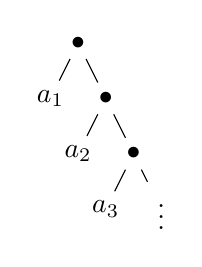
\begin{tikzpicture}[sibling distance=2em, level distance=2em]
  \node {\(\bullet\)}
    child { node {\(a_1\)} }
    child { node {\(\bullet\)}
      child { node {\(a_2\)}}
      child { node {\(\bullet\)}
        child { node {\(a_3\)}}
        child { node {\(\vdots\)}
    }}};
\end{tikzpicture}
\qquad
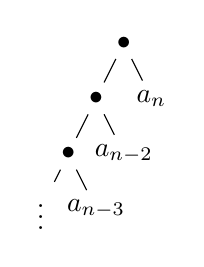
\begin{tikzpicture}[sibling distance=2em, level distance=2em]
  \node {\(\bullet\)}
    child { node {\(\bullet\)}
      child { node {\(\bullet\)}
        child {node {\(\vdots\)}}
        child {node {\(a_{n-3}\)}}}
      child { node {\(a_{n-2}\)}}
        }
    child { node {\(a_n\)} };
\end{tikzpicture}
\qquad
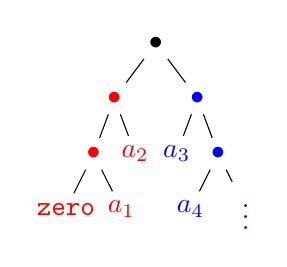
\begin{tikzpicture}[level distance=2em, level 3/.style={sibling distance=2em}, level 2/.style={sibling distance=1.5em}, level 1/.style={sibling distance=3em}]
  \node {\(\bullet\)}
  child { node[color=red] {\(\bullet\)}
    child { node[color=red] {\(\bullet\)}
      child {node[color=red] {\texttt{zero}}}
      child {node[color=red] {\(a_1\)}}}
    child { node[color=red] {\(a_2\)}}
  }
  child { node[color=blue] {\(\bullet\)}
    child { node[color=blue] {\(a_3\)} }
    child { node[color=blue] {\(\bullet\)}
      child { node[color=blue] {\(a_4\)}}
      child { node[color=blue] {\(\vdots\)}
      }}};
\end{tikzpicture}
\end{center}

\begin{block}{Quiz}
  Can we swap the two red branches in the last tree?
\end{block}
\end{frame}

\begin{frame}[fragile] \frametitle{LARGER USE CASES}
  \framesubtitle{Parallelization}

  \begin{block}{}
  \begin{lstlisting}
object Parallel {

  def mconcat[A:Monoid](as: Traversable[A]): A =
    ~\alt<1>{as.foldLeft(Monoid[A].zero)(\_ |+| \_)}{}\alt<2>{as.\alert{fold}(Monoid[A].zero)(\_ |+| \_)}{}\alt<3->{as.\textcolor{blue}{par}.\alert{fold}(Monoid[A].zero)(\_ |+| \_)}{}~
}
  \end{lstlisting}
  \end{block}

  \invisible<1>{
    \texttt{fold[A1 >: A](z: A1)(op: (A1, A1) => A1): A1}
    \vspace{2ex}

    \texttt{z}: a \alert{neutral} element for the fold operation;
    may be added to the result an arbitrary number of times, and \alert{must not change the result.}

    \texttt{op}: a binary operator that must be \alert{associative.}
    \begin{block}{}
      \centering
      \large \textbf{But, but... That's just a Monoid!}
    \end{block}
  }
\end{frame}

\begin{frame}[fragile] \frametitle{LARGER USE CASES}
  \framesubtitle{Parallelization}
  \begin{itemize}
    \item You could have \emph{invented} the Monoid trying to write a parallel \texttt{fold}.
    \item This is how you \emph{discover} the laws for an algebraic structure.
    \item If you have a Monoid, you can \alert{fold it in parallel.}
    \item But pay attention to the \alert{monoid laws!!!}
    \item Huge performance win (in certain situations).
    \item Base of several parallel and distributed frameworks.
  \end{itemize}

\end{frame}


\begin{frame} \frametitle{LARGER USE CASES}
  \framesubtitle{Incremental updates}
  \begin{block}{The Problem}
    \begin{itemize}
      \item System measures a magnitude (e.g. latency)
      \item Compute and store daily means, variances, etc.
      \item Events arrive at high rate (millions per hour)
    \end{itemize}
  \end{block}


\end{frame}

\begin{frame} \frametitle{LARGER USE CASES}
  \framesubtitle{Incremental updates}
  \begin{columns}[c]
    \column{0.6\textwidth}
      \begin{block}{Naive approach}
        \begin{itemize}
        \item On each measurement load all history,
        \item recompute mean/variance/etc.,
        \item store.
        \end{itemize}
      \end{block}

    \column{0.3\textwidth}
  Too much \alert{memory}, to much compute \alert{time}, not able to \alert{catch up}
  to the stream.
  \end{columns}

  \pause

  \begin{columns}[c]
    \column{0.6\textwidth}
      \begin{block}{Unsound approach}
        \begin{itemize}
        \item Store previous mean/variance,
        \item on measurement average previous and current,
        \item store.
        \end{itemize}
      \end{block}

    \column{0.3\textwidth}
    Fast, low memory, but \alert{incorrect}.
    \begin{align*}
      \mu[1,0,0] & = 1/3 \\
      \mu[\mu[1,0], 0] &= 1/4
    \end{align*}

  \end{columns}
\end{frame}

\begin{frame} \frametitle{LARGER USE CASES}
  \framesubtitle{Incremental updates}
  \begin{block}{A better approach}
  \begin{itemize}
    \item Find a \alert{Monoid for mean/variance/etc} of \(n\) samples.
    \item Serialize the Monoid to storage.
    \item Accumulate several (or 1) new measurements.
    \item \alert{Combine} the old and new results using the monoid.
    \item Store.
  \end{itemize}
  \end{block}

  \pause

  \begin{block}{How is it better?}
  \begin{itemize}
    \item \alert{Exact} if we can find the right Monoid.
    \item \alert{\(O(1)\) updates} (independent of sample size).
    \item Trade off performance for freshness.
  \end{itemize}
  \end{block}

\end{frame}

\begin{frame} \frametitle{LARGER USE CASES}
  \framesubtitle{Incremental updates}
  What to store?
  \begin{block}{Weighted average of the means}
    \[
    \begin{split}
      n\cdot \mu = \sum_{i=0}^{n-1} x_i \qquad  m\cdot \nu = \sum_{i=0}^{m-1} x_{i+n} \\
      \frac{1}{n+m} \sum_{i=0}^{n+m-1} x_i = \frac{n\mu + m\nu} {n+m}
    \end{split}
    \]
  \end{block}

  We need previous \alert{mean} and \alert{sample size.}

  Generalizing, to compute the nth-moment, we need to store n+1 values.
\end{frame}

\begin{frame}[fragile] \frametitle{LARGER USE CASES}
  \framesubtitle{Incremental updates}
  \begin{block}{A data type for mean and variance}
  \begin{lstlisting}
sealed abstract class MeanVar

final case object EmptyMeanVar extends MeanVar

final case class MeanVarV(
  m1: Double,
  m2: Double,
  n: Long) extends MeanVar
  \end{lstlisting}
  \end{block}
\end{frame}

\begin{frame}[fragile] \frametitle{LARGER USE CASES}
  \framesubtitle{Incremental updates}
  \begin{block}{Utility functions: creating \texttt{MeanVars}}
  \begin{lstlisting}
object MeanVar {

  def singleton(x: Double): MeanVar = MeanVarV(x, 0, 1)

  def sample(xs: Traversable[Double]): MeanVar = ~\pause~
    foldMap(singleton(_))(xs)
}
  \end{lstlisting}
  \end{block}
\end{frame}

\begin{frame}[fragile] \frametitle{LARGER USE CASES}
  \framesubtitle{Incremental updates}
  \begin{block}{Utility functions: extracting from \texttt{MeanVars}}
  \begin{lstlisting}
object MeanVar {
  def sampleSize: MeanVar => Long = {
    case MeanVarV(_, _, n) => n
    case _ => 0
  }
  def mean: MeanVar => Option[Double] = {
    case MeanVarV(m1, _, _) => Some(m1)
    case _ => None
  }
  def variance: MeanVar => Option[Double] = {
    case MeanVarV(_, _, 1) => Some(0)
    case MeanVarV(_, m2, n) => Some(m2/(n - 1.0))
    case _ => None
  }
}
  \end{lstlisting}
  \end{block}
\end{frame}

\begin{frame}[fragile] \frametitle{LARGER USE CASES}
  \framesubtitle{Incremental updates}
  \begin{block}{The Monoid}
  \begin{lstlisting}
val meanVarMonoid: Monoid[MeanVar] = new Monoid[MeanVar] {
  def zero: MeanVar = EmptyMeanVar

  def append(a: MeanVar, b: => MeanVar): MeanVar = (a, b) match {
    case (EmptyMeanVar, a) => a
    case (a, EmptyMeanVar) => a ~\pause~
    case (MeanVarV(m1a, m2a, na), MeanVarV(m1b, m2b, nb)) => {
      val nt = na + nb
      val delta = m1b - m1a
      MeanVarV(~\alert{(na * m1a + nb * m1b ) / nt}~,
                m2a + m2b + delta * delta * na * nb / nt,
                ~\alert{nt}~)
    }
  }
}
  \end{lstlisting}
  \end{block}
\end{frame}

\begin{frame}[fragile] \frametitle{LARGER USE CASES}
  \framesubtitle{Incremental updates}
  \begin{block}{Updating the statistics (pseudocode)}
  \begin{lstlisting}
     // Define a time resolution (accumulate for 1sec? 100ms?)
     val newData: Vector[Double] = getNewMeasurements(...)

     // Compute mean/var of the new data (incremental work)
     val newStats: MeanVar = MeanVar.sample(newData)

     // This is an O(1) op
     // In our example this loads 3 numbers,
     // doesn't matter how many samples we have processed before
     val oldStats: MeanVar = loadStats(...)

     // Another O(1) operation
     storeStats(oldStats |+| newStats)
  \end{lstlisting}
  \end{block}
\end{frame}


\begin{frame} \frametitle{LARGER USE CASES}
  \framesubtitle{Incremental updates}
  \begin{itemize}
    \item You could have \emph{invented} the Monoid trying to write incremental updates.
    \item This is how you \emph{discover} the laws for an algebraic structure.
    \item Didn't we say \texttt{Double} under \texttt{(+)} is not a Monoid?
    \item Extensible to higher momenta.
    \item Extensible to approximate histograms and other fun stuff.
  \end{itemize}
  \begin{block}{Take-home quiz}
    \begin{itemize}
    \item How can we do rolling averages? We would need to \emph{delete} the older
    accumulated data.
    \item Write two different Monoids for \texttt{Map[K, V]}. Do you need to
      impose restrictions on \texttt{V}?
    \end{itemize}
  \end{block}
\end{frame}

\subsection*{References}
\begin{frame} \frametitle{REFERENCES}
  \begin{columns}[c]
    \column{0.7\textwidth}
      \begin{itemize}

        \item This talk: slides, all the \alert{code and many tests} \\
          \href{https://github.com/paraseba/}{\underline{https://github.com/paraseba/}} % fixme

        \item \textit{Functional Programming in Scala.}\\ Paul Chiusano \& Runar Bjarnason

        \item \textit{Why Functional Programming Matters} \\
          John Hughes.

        \item \textit{Computing skewness and kurtosis in one pass.} \\
          {\footnotesize \href{https://www.johndcook.com/blog/skewness\_kurtosis/}{\underline{https://www.johndcook.com/blog/skewness\_kurtosis/}}}

        \item Scalaz library \\
          {\href{https://github.com/scalaz/scalaz}{\underline{https://github.com/scalaz/scalaz}}}
      \end{itemize}

    \column{0.3\textwidth}

    \begin{figure}
        \centering
        \includegraphics[width=\textwidth]{functional-programming-in-scala.png}
    \end{figure}
  \end{columns}
\end{frame}

\section{Monoids in Design \color[rgb]{0.5,0.1,0.9}[next session]}

\begin{frame}{ToDo}
\end{frame}


% \begin{frame}{ToDo / Fixme}
%   \begin{itemize}
%     \item what happens with broken rules
%     \item Monoid seems too simple but it's powerful
%     \item mconcat can be parallelized, incrementally, cached
%     \item dual monoid
%     \item summaries
%     \item substracition not a monoid
%     \item where to find code/presentation
%     \item mathematical building, is elegant, if you don't care about
%           elegance in software what do you care about? elegance is simple (not easy)
%     \item accent
%     \item quizes to keep awake
%     \item grammarly
%     \item lazyness, is the by name argument important?
%     \item integer overflow is a monoid?
%     \item either monoid?
%     \item monoid for config
%     \item grothendieck on finding the right level of abstraction
%     \item mconcat can't be defined properly without associativity
%     \item mention semigroup
%     \item using equality when defining monoids for functions, what it means
%       equal functions
%     \item monoids capture *the escence* of combining things associatively
%     \item laws must be probed by hand, type system not enough
%     \item topic for design session: aggregations (a la beautiful folds)
%       \item add filter as example of foldMap
%         \item use palette colors
%   \end{itemize}
% \end{frame}

\end{document}